\section{White Rabbit extension to PTP (WRPTP)}
\label{sec:wrptp}

White Rabbit extends the PTP standard benefiting from PTP's mechanisms, 
taking advantage of its customization facilities (i.e. PTP profiles
and Type-Length-Value, TLV) but also defining implementation-specific 
functionalities and staying PTP-compatible. 

% \begin{figure}[!t]
% \centering
% 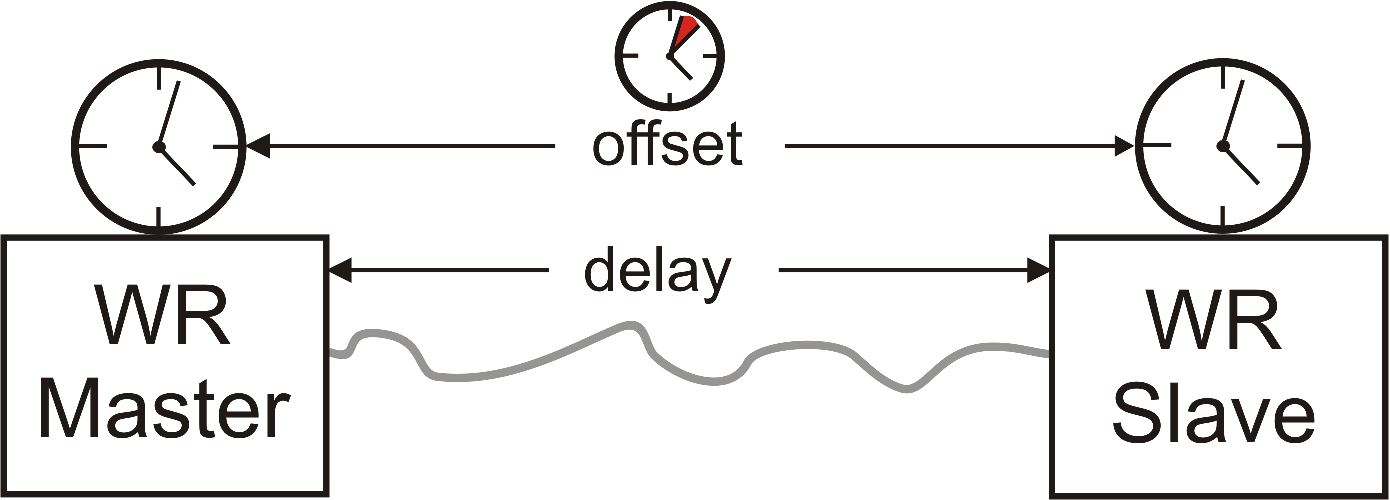
\includegraphics[width=3in]{fig/wrLink.eps}
% \caption{WR Link \modified{Delay} Model, synchronization and syntonization scheme.}
% \label{fig:wrLink}
% \end{figure}

\begin{figure}[!t]
\centering
\includegraphics[width=3.15in]{../../figures/protocol/wrptpMSGs.eps}
\caption{\modified{Simplified overview of the message flow in WRPTP.}}
\label{fig:wrptpMSGs}
\end{figure}

WRPTP introduces the \textit{WR Link Setup} (section~\ref{sec:wrLinkSetup}) process which
provides inputs to the \textit{WR Link \modified{Delay} Model} (section~\ref{sec:wrLinkModel}) 
to obtain accurate delay and offset calculations. 
The WR Link Setup is a process for establishing the WR link. It includes WR node
identification, syntonization, measurement of WR-specific parameters and 
their distribution over the link. The additional communication during the WR Link Setup 
is done through extended PTP messaging facilities (section~\ref{sec:wrMessages}). 
The WR-specific parameters, which are exchanged and set during this process, are 
stored in WR-specific data set fields (section~\ref{sec:wrDataSet}). 

The flow of events for the standard PTP is extended as depicted in \figurename~\ref{fig:wrptpMSGs}
and described below:

\begin{enumerate}
\item \textbf{WR Port A} which is in PTP\_MASTER state periodically sends WR Announce messages
      (section~\ref{sec:wrMessages}).
\item \textbf{WR Port B} receives Announce message(s), recognizes the WR Announce message and 
      uses the modified Best Master Clock (mBMC) algorithm (section~\ref{sec:wrBMC}) to establish its
      place in the WR network hierarchy.
\item \textbf{WR Port B} enters WR Slave mode (based on the conditions in 
      \ref{sec:wrLinkSetup}) and starts the WR Link Setup by sending the M\_SLAVE\_PRESENT message.
\item \textbf{WR Port A} enters WR Master mode (based on the conditions in 
      \ref{sec:wrLinkSetup}) and sends the M\_LOCK message to request the WR Slave to start
      syntonization.
\item The WR Slave sends the M\_LOCKED message as soon as the syntonization process is 
      finished.
\item The WR Master sends the M\_CALIBRATE message to request a calibration pattern in order to 
      measure its reception fixed delay.
\item The WR Master sends the M\_CALIBRATED message as soon as the calibration is 
      finished.
\item The WR Slave sends the M\_CALIBRATE message to request a calibration pattern in order to 
      measure its reception fixed delay.
\item The WR Slave sends the M\_CALIBRATED message as soon as the calibration is 
      finished.
\item The WR Master sends the M\_WR\_MODE\_ON message to indicate completion of  the WR
      Link Setup process.
\item PTP two-step clock request-response delay measurement is performed repeatedly ($t_{1}$,
      $t_{2}$, $t_{3}$, $t_{4}$). WR Slave calculates M-to-S delay and clock offset and adjusts its
      time counters.
\end{enumerate}

% \begin{figure}[!t]
% \centering
% \includegraphics[width=3.5in]{fig/wrptpMSGs.eps}
% \caption{\modified{Simplified overview of the message flow in WRPTP.}}
% \label{fig:wrptpMSGs}
% \end{figure}

\begin{figure}[!t]
\centering
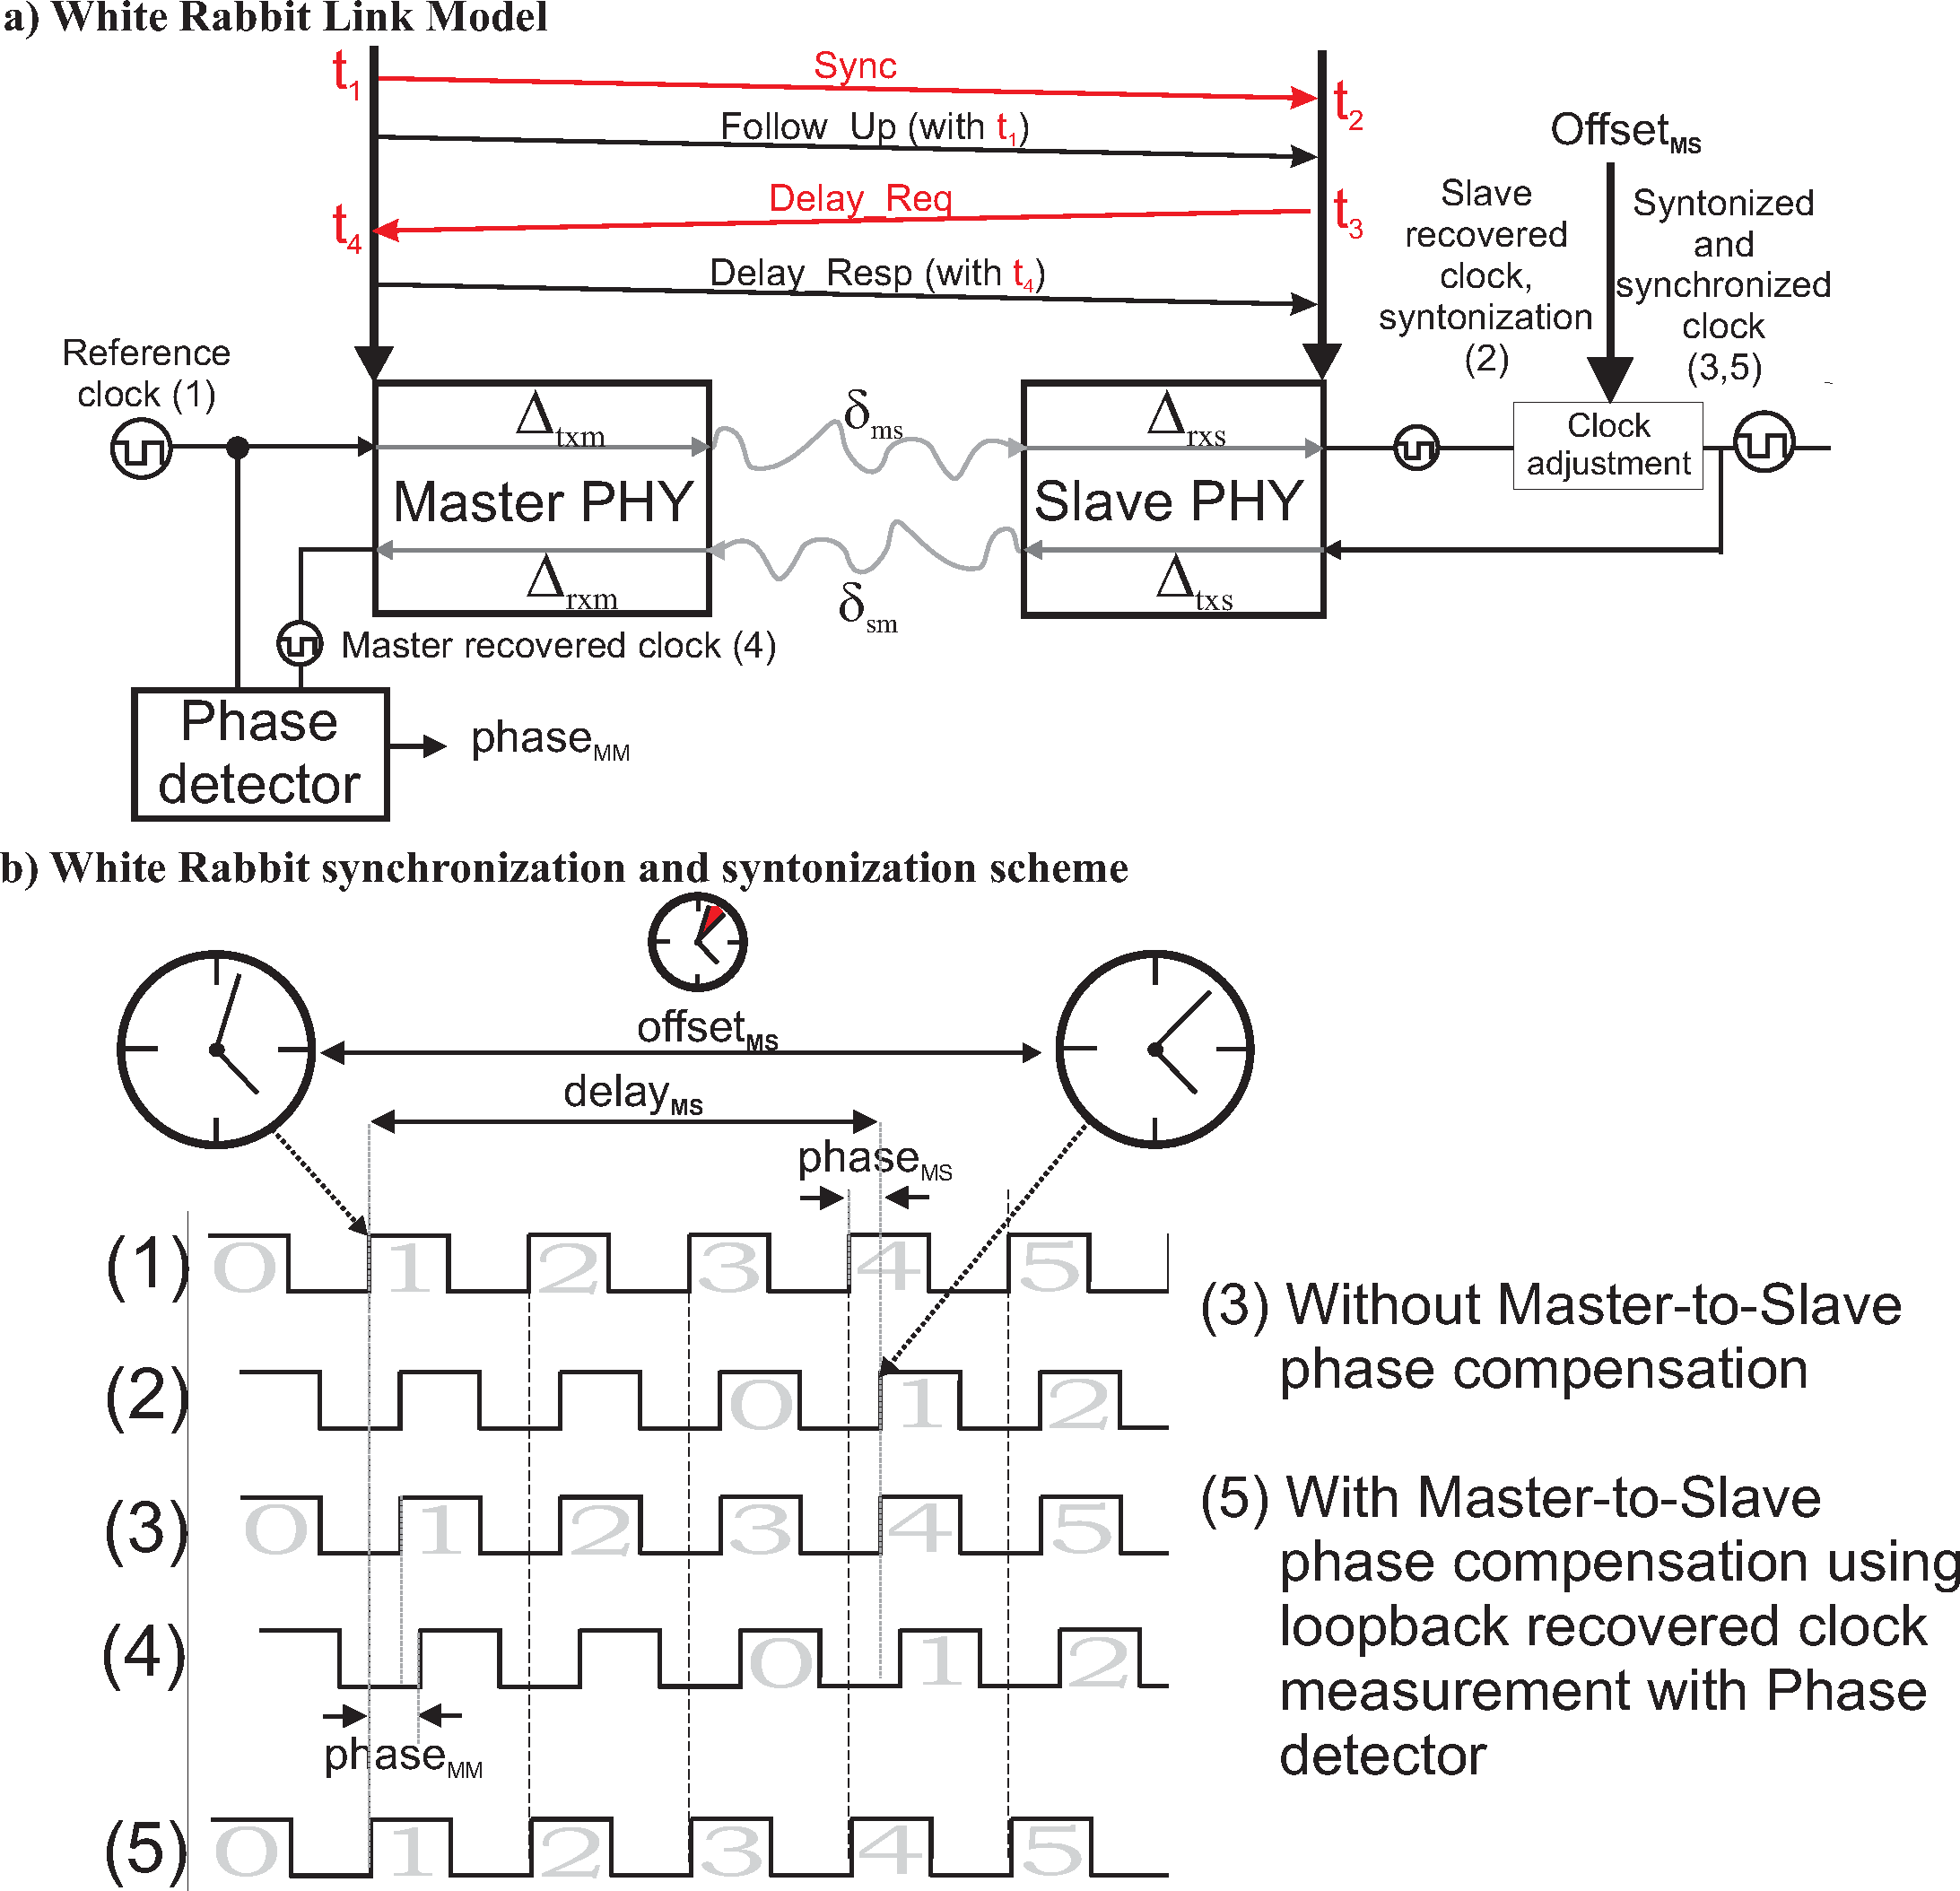
\includegraphics[width=3.1in]{../../figures/protocol/wrLink2.eps}
\caption{WR Link \modified{Delay} Model, synchronization and syntonization scheme.}
\label{fig:wrLink}
\end{figure}



%%%%%%%%%%%%%%%%%%%%%%%%%%%%%%%%%%%%%%%%%%%%%%%%%%%%%%%%%%%%%%%%%%%%%%%%%%%%%%%
%             WR Link Delay Model
%%%%%%%%%%%%%%%%%%%%%%%%%%%%%%%%%%%%%%%%%%%%%%%%%%%%%%%%%%%%%%%%%%%%%%%%%%%%%%%

\subsection{WR Link \modified{Delay} Model}
\label{sec:wrLinkModel}
Sub-nanosecond synchronization requires a precise knowledge of one-way 
M-to-S delay ($ delay_{ms}$). PTP measures 
the round-trip delay ($delay_{MM}$). Usually, delay symmetry 
($delay_{ms}=delay_{sm}$) is assumed to derive the one-way delay. In
White Rabbit, the \textit{WR Link \modified{Delay} Model} (\figurename~\ref{fig:wrLink}, (a)) 
is used to calculate the precise M-to-S delay by including link asymmetry. 
The delay can be expressed as the sum:
\begin{equation}
  \label{eq:delayms}
  delay_{ms} = \Delta_{tx_m} + \delta_{ms} + \Delta_{rx_s}
\end{equation}
where $\Delta_{tx_m}$ is the fixed delay due to the master's
transmission circuitry, $\delta_{ms}$ is the variable delay of the
transmission medium and $\Delta_{rx_s}$ is the fixed circuitry
reception delay in the slave. Similarly, the S-to-M
delay ($ delay_{sm}$) can be described using $\Delta_{tx_s}$,
$\delta_{sm}$ and $\Delta_{rx_m}$ respectively. The fixed delays
($\Delta_{rx_s,tx_s,rx_m,tx_m}$) are considered constant for a given
connection. They can be measured by nodes/switches at the beginning of 
the connection, as described in section~\ref{sec:TxRxLatencies}. For
highest precision, WR uses a single fiber for two-way
communication -- the asymmetry is directly and solely caused
by the difference in propagation velocity in both directions. Consequently, the
difference between $\delta_{ms}$ and $\delta_{sm}$ is connected to the
wavelength difference for transmitting and receiving the data
(e.g. 1550 and 1310 nm). The equation describing the relation between
$\delta_{ms}$ and $\delta_{sm}$ is defined in \cite{biblio:WRPTP}.
For bi-directional fiber, it is governed by the 
\textit{relative delay coefficient~($\alpha$)}:
\begin{equation}
  \label{eq:alpha}
  \alpha = \frac{\delta_{ms}}{\delta_{sm}}-1 = \frac{n_{1550}}{n_{1310}}-1
\end{equation}
The $\alpha$ coefficient can be calculated using refractive indexes
($n_{1550}$, $n_{1310}$) or, preferably, measured for a given fiber type. 

Knowing the coefficient, the round-trip delay ($delay_{MM}$)
and the fixed delays ($\Delta_{rx_s,tx_s,rx_m,tx_m}$), 
the precise M-to-S delay (\ref{eq:delayMS}) can be calculated using (\ref{eq:delta}) and
(\ref{eq:ptpTimestamps}). See \cite{biblio:WRPTP} and
\cite{biblio:TomekMSc} for a detailed derivation.
\begin{equation}
\label{eq:delta}
  \Delta = \Delta_{tx_m} + \Delta_{rx_s} + \Delta_{tx_s} + \Delta_{rx_m}
\end{equation}
\begin{equation}
\label{eq:ptpTimestamps}
  delay_{MM} =  \Delta + \delta_{ms} +\delta_{sm}
\end{equation}
\begin{equation}
\label{eq:delayMS}
  delay_{ms} = \frac{1 + \alpha}{2 + \alpha}(delay_{MM}-\Delta)
\end{equation}
Finally, the value of the offset ($offset_{ms}$) between the master's
clock and that of the slave is obtained (\ref{eq:offset}). It is fed
into the adjustment algorithm of the slave's clock servo
(\figurename~\ref{fig:wrLink}).
\begin{equation}
\label{eq:offset}
  offset_{ms} = t_1-t_{2p} - delay_{ms}
\end{equation}
The $t_{2p}$ in (\ref{eq:offset}) is the enhanced-precision value of PTP $t_2$ 
which is obtained during the \textit{Fine Delay Measurement} described
in section~\ref{sec:fineDelay}. The same process is used to obtain a very precise
value of $t_{4}$.
% The fixed delays ($\Delta_{rx_s,tx_s,rx_m,tx_m}$) measurement is described in 
% section~\ref{sec:TxRxLatencies}.

% \modified{The link asymmetry, thus the precise one-way delay, 
% is re-evaluated periodically each time new PTP-timestamps are obtained. It enables to compensate for 
% the possible changes of the link characteristics.}
%The application of the \textit{WR Link \modified{Delay} Model} needs extensions to the
%PTP standard which are described in the next sub-section.


%%%%%%%%%%%%%%%%%%%%%%%%%%%%%%%%%%%%%%%%%%%%%%%%%%%%%%%%%%%%%%%%%%%%%%%%%%%%%%%
%             WR Data Sets
%%%%%%%%%%%%%%%%%%%%%%%%%%%%%%%%%%%%%%%%%%%%%%%%%%%%%%%%%%%%%%%%%%%%%%%%%%%%%%%

\subsection{WR Data Sets}
\label{sec:wrDataSet}

WRPTP adds fields to the data sets defined in the PTP standard 
%(\tablename~\ref{tab:wrDS}) % table excluded from article due to the lack of space and uselessnes
and defines a new data set (backupParentDS) to store WR-specific parameters. All new fields, except
\textit{primarySlavePortNumber}, are added to the \textit{portDS} data set. 
The \textit{primarySlavePortNumber} field is added to the \textit{currentDS} data set.

% \begin{table}[!t]
% %\renewcommand{\arraystrech}{1.3}
% \caption{WRPTP data sets fields (\textbf{D}=Dynamic, \textbf{S}=Static).}
% \label{tab:wrDS}
% \centering
% \begin{tabular}{| l     |     c         |  l |   }        \hline   
%    
% \textbf{DS member}     	&  \textbf{D}/\textbf{S} & \textbf{Description}\\   \hline
% %			&   &                \\ \hline
% %%%%%%%%%%%%%%%%%%%%%%%%%%%%%%%%%%%%%%%%%%%%%%%%%%%%%%%%%%%%%%%%%%%%%%%%%%%%%%%%%%%%%%%%%%
% wrConfig   		& S & predefined function of a WR port \\ \hline
% wrMode			& D & current WR mode of a WR port	 \\ \hline
% wrModeOn 		& D & mode defined in wrMode is active \\ \hline
% wrPortState 		& D & current state of the WR FSM      \\ \hline
% calibrated 		& D & fixed delays of the given port   \\ \hline
% deltaTx       		& D & port's $\Delta_{tx}$             \\ \hline
% deltaRx     		& D & port's $\Delta_{rx}$             \\ \hline
% calPeriod   		& S & calibration period\\ \hline
% %%%%%%%%%%%%%%%%%%%%%%%%%%%%%%%%%%%%%%%%%%%%%%%%%%%%%%%%%%%%%%%%%%%%%%%%%%%%%%%%%%%%%%%%%%
% parentWrConfig 		& D & wrConfig of the parent port\\ \hline
% parentWrMode		& D & wrMode of the parent port\\ \hline
% parentWrModeOn 		& D & wrModeOn of the parent port\\ \hline
% parentDeltaTx      	& D & calibrated of the parent port\\ \hline
% parentDeltaRx     	& D & deltaTx of the parent port\\ \hline
% parentCalPeriod   	& S & deltaRx of the parent port\\ \hline
% %%%%%%%%%%%%%%%%%%%%%%%%%%%%%%%%%%%%%%%%%%%%%%%%%%%%%%%%%%%%%%%%%%%%%%%%%%%%%%%%%%%%%%%%%%
% primarySlavePortNumber	&  D &port number of the Primary Slave  \\ \hline
% 
% \end{tabular}
% 
% \end{table}

%%%%%%%%%%%%%%%%%%%%%%%%%%%%%%%%%%%%%%%%%%%%%%%%%%%%%%%%%%%%%%%%%%%%%%%%%%%%%%%
%             WR Messages
%%%%%%%%%%%%%%%%%%%%%%%%%%%%%%%%%%%%%%%%%%%%%%%%%%%%%%%%%%%%%%%%%%%%%%%%%%%%%%%

\subsection{WR Messages}
\label{sec:wrMessages}

WRPTP defines a WR Type-Length-Value (WR TLV) extension to exchange the WR-specific data.
In particular, it is used to suffix Announce and create Signaling Messages. 
WR TLVs are recognized (see \tablename~35 of PTP) by the TLV type
(\textit{tlvType}=\textit{ORGANIZATION\_EXTENSION}), CERN's Organizationally Unique Identifier 
(\textit{OrganizationId} = 0x080030), magic and version numbers. The different types of WR
TLVs are distinguished by a WR Message Identifier (wrMessageID), as defined in
\tablename~\ref{tab:wrMessageId}.

\begin{table}[!t]
\caption{White Rabbit Message ID values}
\centering
\begin{tabular}{| l | c| c | c |}          \hline
\textbf{Message name}  &  \textbf{wrMessageId} &  \textbf{Sent in message type} \\   \hline
%& &  \\ \hline
M\_SLAVE\_PRESENT     &  0x1000 & Signaling \\ \hline
M\_LOCK               &  0x1001 & Signaling \\ \hline
M\_LOCKED             &  0x1002 & Signaling \\ \hline
M\_CALIBRATE          &  0x1003 & Signaling \\ \hline
M\_CALIBRATED         &  0x1004 & Signaling \\ \hline
M\_WR\_MODE\_ON       &  0x1005 & Signaling \\ \hline
M\_ANN\_SUFIX	      &  0x2000 & Announce  \\ \hline
\end{tabular}
\label{tab:wrMessageId}
\end{table}

%%%%%%%%%%%%%%%%%%%%%%%%%%%%%%%%%%%%%%%%%%%%%%%%%%%%%%%%%%%%%%%%%%%%%%%%%%%%%%%
%             WR Messages
%%%%%%%%%%%%%%%%%%%%%%%%%%%%%%%%%%%%%%%%%%%%%%%%%%%%%%%%%%%%%%%%%%%%%%%%%%%%%%%

\subsection{Modified BMC}
\label{sec:wrBMC}
The standard method of handling topology and grandmaster redundancy in a BC-based PTP network 
is not sufficient for the WRN. The BMC allows only a single port (slave) of a BC to 
be synchronized to a single grandmaster. A time source failure requires re-synchronization and might
introduce fluctuations in the notion of time.

% The BMC allows no more than one port of a BC to be in the PTP\_SLAVE state. Such a
% solution allows for redundancy of the time source and topology but is not optimal for the
% continuity of the synchronization. In case of a failure of one of the \textit{best}
% clocks, the restart of the estimation of the clock drift, mean path delay and offset is required
% which might cause fluctuations in the notion of time. 
 
The modified BMC (mBMC) allows for more than one \textit{best} clock in a single domain, 
enabling the creation of a logic topology with multiple roots. A BC 
running the mBMC can have more than one port in the PTP\_SLAVE state (slave ports). 
This means that timing information is exchanged between a BC and 
more than one source of time (i.e. OC or BC). At any time 
any of these sources can be used to perform synchronization, including a weighted 
average from all slave ports as mentioned in \cite{biblio:Takahide}.

The modification applies to the State Decision Algorithm (SDA): the BMC\_SLAVE 
recommended state is enforced instead of the BMC\_PASSIVE state 
\modified{for the clocks with clockClass greater than 127 \cite{biblio:IEEE1588}}. A port
which becomes a slave as a result of the modification, is considered
a Secondary Slave. A slave port resulting from the unchanged part of the SDA,
is considered a Primary Slave and its number is stored in the \textit{primarySlavePortNumber}. 

The best qualified Announce messages ($E_{rbest}$) 
from all Secondary Slave ports are compared using the Data Comparison Algorithm (DCA) 
to determine the "second best master" and the lower order masters. The results 
are stored in the \textit{backupParentDS} \modified{(section~\ref{sec:wrDataSet})}.

The provided information about Primary and Secondary Slaves is used by the WR hardware
to support a seamless switch-over in case of failure of the best master 
(section~\ref{sec:wrCRS}). \modified{Such a solution enables robust synchronization with no 
deterioration of its quality while switching between the redundant components.}
%%%%%%%%%%%%%%%%%%%%%%%%%%%%%%%%%%%%%%%%%%%%%%%%%%%%%%%%%%%%%%%%%%%%%%%%%%%%%%%
%             Link Setup
%%%%%%%%%%%%%%%%%%%%%%%%%%%%%%%%%%%%%%%%%%%%%%%%%%%%%%%%%%%%%%%%%%%%%%%%%%%%%%%

\subsection{WR Link Setup}
\label{sec:wrLinkSetup}

The process of establishing a White Rabbit link between two WR ports
is called \textit{WR Link Setup}. It involves the
recognition of two compatible WR ports, their WR modes assignment
(WR Master or WR Slave), syntonization over the physical layer, 
measurement of the fixed delays ($\Delta_{rx_s,tx_s,rx_m,tx_m}$) and 
exchange of their values across the link. The WR Link Setup is controlled by the
White Rabbit state machine (WR FSM) which is executed in the PTP\_UNCALIBRATED 
state of the PTP FSM \modified{on the WR Slave, and in the PTP\_MASTER state on the WR Master}. 
The WR FSM is depicted in \figurename~\ref{fig:wrFSM} and 
its usual execution on the WR Master and the WR Slave during the WR Link Setup is
presented in \figurename~\ref{fig:wrptpMSGs}.
%%%%%%%%%%%%%%%%%%%%%%%%%%%%%%%%%%%%%%%%%%%%%%%%%%%%%%%%%%%%%%%%%%%%%%%%%%%%%%%
\begin{figure}[!t]
\centering
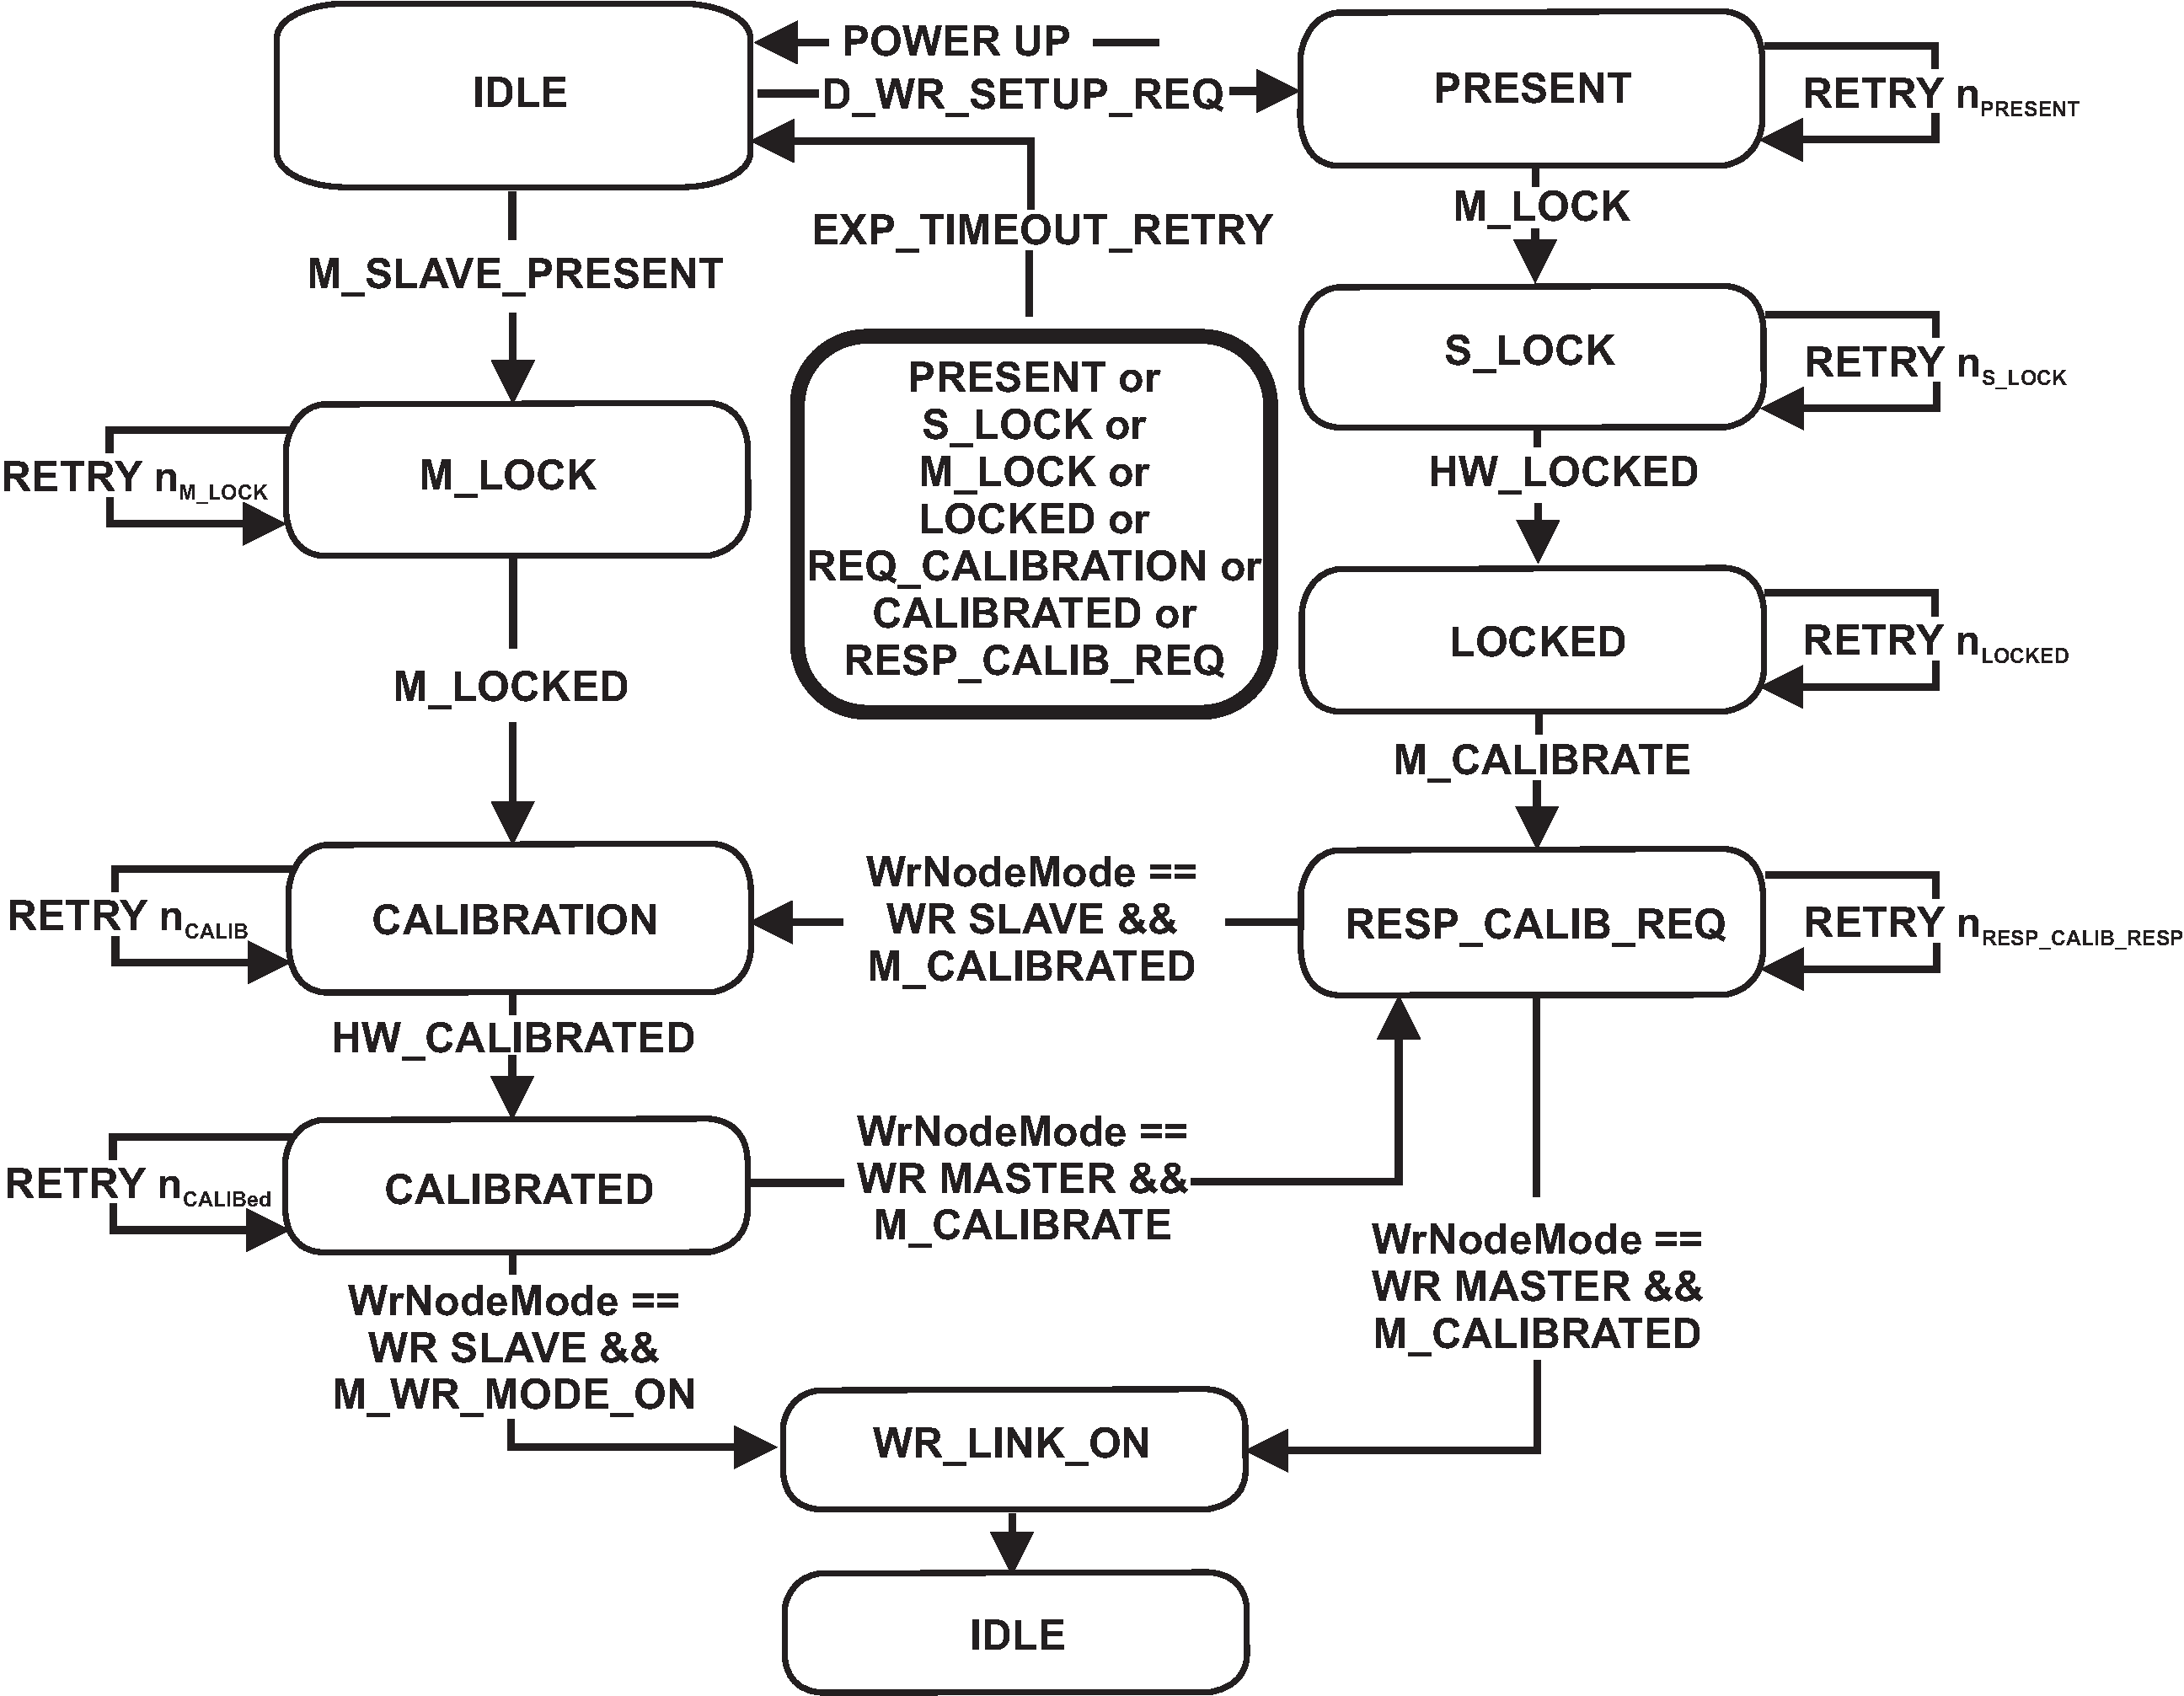
\includegraphics[width=3.1in]{../../figures/protocol/wrFSM.eps}
\caption{\modified{WR state machine \cite{biblio:WRPTP}.}}
\label{fig:wrFSM}
\end{figure}
%%%%%%%%%%%%%%%%%%%%%%%%%%%%%%%%%%%%%%%%%%%%%%%%%%%%%%%%%%%%%%%%%%%%%%%%%%%%%%%

A WR port can become a WR Master, Slave or enter non-WR mode depending on its 
place in the network hierarchy (mBMC's outcome) and WR-specific parameters. 
The following conditions need to be fulfilled by a WR port 
to enter the WR Slave mode and start the WR Link Setup by entering the PRESENT state of the WR FSM
(\figurename~\ref{fig:wrptpMSGs} \& \figurename~\ref{fig:wrFSM}: \textit{D\_WR\_SETUP\_REQ}):
\begin{itemize}
\item the port is not in the PTP\_SLAVE state \textbf{AND}
\item the port is WR Slave-enabled \textbf{AND}
\item the mBMC's Recommended State is BMC\_SLAVE \textbf{AND}
\item the parent port is WR Master-enabled \textbf{AND}
\item at least one of the ports on the link is not in active WR mode.
\end{itemize}
Similarly, the following conditions need to be fulfilled by a WR port 
to become the WR Master and start the WR Link Setup by entering the S\_LOCK state of the WR FSM
(\figurename~\ref{fig:wrptpMSGs}):
\begin{itemize}
\item the port is in the PTP\_MASTER state \textbf{AND}
\item the port is WR Master-enabled \textbf{AND}
\item the M\_SLAVE\_PRESENT message has been received.
\end{itemize}

On successful completion of the \textit{WR Link Setup} the WR mode (wrMode) 
of a port is validated by setting \\ wrModeOn~=~TRUE. 



%%%%%%%%%%%%%%%%%%%%%%%%%%%%%%%%%%%%%%%%%%%%%%%%%%%%%%%%%%%%%%%%%%%%%%%%%%%%%%%
%             WR PTP Profile
%%%%%%%%%%%%%%%%%%%%%%%%%%%%%%%%%%%%%%%%%%%%%%%%%%%%%%%%%%%%%%%%%%%%%%%%%%%%%%%

\subsection{WRPTP Profile}

\begin{table}[!t]
\caption{WRPTP profile.}
\centering
\begin{tabular}{| c | p{5cm} |}          					\hline
%\multicolumn{2}{|c|}{\textbf{PTP Profile}}  				  \\ \hline
profleName           &  White Rabbit     				  \\ \hline
profileVersion       &  1.0               				  \\ \hline
profileIdentifier    &  08-00-03-00-01-00 				  \\ \hline
organizationName     &  European Organization for Nuclear Research (CERN) \\ \hline
sourceIdentification &  http://www.ohwr.org/projects/white-rabbit         \\ \hline
\end{tabular}
\label{tab:wrPtpProfile}
\end{table}


The White Rabbit PTP profile defines the profile's identification 
(\tablename~\ref{tab:wrPtpProfile}). It specifies the values of some of the parameters
(e.g. priority1, logSyncInterval) and the options to be used. 
It indicates the delay request-response mechanism as the only one used by
the WRPTP. It also specifies the mBMC to be used and the WR TLV to be supported.






